% Options for packages loaded elsewhere
\PassOptionsToPackage{unicode}{hyperref}
\PassOptionsToPackage{hyphens}{url}
\documentclass[
  11pt,
]{article}
\usepackage{xcolor}
\usepackage[margin=1in]{geometry}
\usepackage{amsmath,amssymb}
\setcounter{secnumdepth}{-\maxdimen} % remove section numbering
\usepackage{iftex}
\ifPDFTeX
  \usepackage[T1]{fontenc}
  \usepackage[utf8]{inputenc}
  \usepackage{textcomp} % provide euro and other symbols
\else % if luatex or xetex
  \usepackage{unicode-math} % this also loads fontspec
  \defaultfontfeatures{Scale=MatchLowercase}
  \defaultfontfeatures[\rmfamily]{Ligatures=TeX,Scale=1}
\fi
\usepackage{lmodern}
\ifPDFTeX\else
  % xetex/luatex font selection
\fi
% Use upquote if available, for straight quotes in verbatim environments
\IfFileExists{upquote.sty}{\usepackage{upquote}}{}
\IfFileExists{microtype.sty}{% use microtype if available
  \usepackage[]{microtype}
  \UseMicrotypeSet[protrusion]{basicmath} % disable protrusion for tt fonts
}{}
\makeatletter
\@ifundefined{KOMAClassName}{% if non-KOMA class
  \IfFileExists{parskip.sty}{%
    \usepackage{parskip}
  }{% else
    \setlength{\parindent}{0pt}
    \setlength{\parskip}{6pt plus 2pt minus 1pt}}
}{% if KOMA class
  \KOMAoptions{parskip=half}}
\makeatother
\usepackage{graphicx}
\makeatletter
\newsavebox\pandoc@box
\newcommand*\pandocbounded[1]{% scales image to fit in text height/width
  \sbox\pandoc@box{#1}%
  \Gscale@div\@tempa{\textheight}{\dimexpr\ht\pandoc@box+\dp\pandoc@box\relax}%
  \Gscale@div\@tempb{\linewidth}{\wd\pandoc@box}%
  \ifdim\@tempb\p@<\@tempa\p@\let\@tempa\@tempb\fi% select the smaller of both
  \ifdim\@tempa\p@<\p@\scalebox{\@tempa}{\usebox\pandoc@box}%
  \else\usebox{\pandoc@box}%
  \fi%
}
% Set default figure placement to htbp
\def\fps@figure{htbp}
\makeatother
\setlength{\emergencystretch}{3em} % prevent overfull lines
\providecommand{\tightlist}{%
  \setlength{\itemsep}{0pt}\setlength{\parskip}{0pt}}
\usepackage{multicol}
\usepackage{booktabs}
\usepackage{caption}
\usepackage{graphicx}
\usepackage{amsmath, amssymb}
\usepackage{bookmark}
\IfFileExists{xurl.sty}{\usepackage{xurl}}{} % add URL line breaks if available
\urlstyle{same}
\hypersetup{
  pdftitle={Predicting Employment Outcomes among Young Adults: Education{,} Well-being{,} and Machine Learning Evidence from PSID-TAS 2023},
  pdfauthor={Quinn Hart},
  hidelinks,
  pdfcreator={LaTeX via pandoc}}

\title{Predicting Employment Outcomes among Young Adults: Education,
Well-being, and Machine Learning Evidence from PSID-TAS 2023}
\author{Quinn Hart}
\date{June 2026}

\begin{document}
\maketitle

\begin{abstract}
This paper asks which individual characteristics predict current employment among young adults, focusing on two domains: subjective well-being and educational attainment. Using the 2023 wave of the Panel Study of Income Dynamics Transition into Adulthood Supplement (PSID-TAS), I construct a binary indicator of current employment for 2{,}434 young adults and relate it to a ten-item well-being index and nine education variables. Four complementary statistical and machine-learning methods---logistic regression, classification trees (CART), random forests, and the LASSO---are applied separately to each domain, and a combined logistic model evaluates whether well-being carries predictive information beyond education. The results are consistent across all four methods: educational characteristics, especially current college enrollment, prior college attendance, and educational expectations, are strong and stable predictors of employment, whereas well-being has essentially no predictive power on its own. The well-being tree produces no splits, its random forest performs no better than a naive majority-class rule, and the LASSO discards every well-being indicator under the conservative penalty. Notably, the well-being coefficient \emph{strengthens} once education is held constant---a suppression pattern---but remains only marginally significant. The findings suggest that, among young adults, human-capital measures dominate psychological well-being in explaining short-run employment status.
\end{abstract}

\vspace{0.5em}

\begin{multicols}{2}

\section{Introduction}
The transition from adolescence into adulthood is a critical period for labor-market attachment. Whether a young adult is working shapes their income trajectory, skill accumulation, and long-run economic security, and aggregate youth employment is a recurring concern for policymakers. Understanding which individual characteristics distinguish employed from non-employed young adults is therefore of both scientific and practical interest.

Two broad domains plausibly relate to early-career employment. The first is \emph{educational attainment}, the canonical measure of human capital. Standard models predict that more schooling, college enrollment, and stronger educational trajectories raise the probability of labor-market participation and employability. The second, less studied domain is \emph{subjective well-being}. A growing literature in economics and psychology argues that well-being---happiness, life satisfaction, sense of purpose, and social connectedness---constitutes a form of ``psychological capital'' that may support motivation, health, and productivity, and could in turn predict employment. At the same time, the causal arrow may run in either direction, and the two domains are themselves correlated, since education and well-being tend to move together.

This paper addresses two questions. First, do well-being and education each predict current employment among young adults? Second, and more sharply, does well-being add predictive value \emph{beyond} education, or is any apparent association between well-being and employment simply a reflection of educational differences? The second question matters because comparing two domains in isolation can be misleading: a variable that looks weak on its own may still contribute once correlated factors are controlled, and a variable that looks strong may be redundant.

To answer these questions I take a predictive-modeling approach rather than a causal one. I apply four methods that differ in their assumptions and outputs---logistic regression for interpretable linear effects, classification trees for interpretable nonlinear structure, random forests for flexible prediction and variable importance, and the LASSO for regularized variable selection---and compare what each reveals about the two domains. I then estimate a combined logistic model and use a nested likelihood-ratio test to assess the incremental contribution of well-being. Because the data are a single cross-section, the analysis is explicitly associational: the goal is to characterize which features predict employment, not to identify causal effects.

The central finding is that education dominates. Across every method, education variables carry strong and stable predictive signal, while well-being does not. The combined model reveals a subtle twist---the well-being coefficient grows after adjusting for education---but the effect remains marginal and economically small. The remainder of the paper describes the data, the empirical strategy, the results for each domain, and the implications and limitations of the analysis.

\section{Data}
The data are drawn from the 2023 wave of the PSID Transition into Adulthood Supplement, which surveys young adults in PSID families. The working file contains 2{,}434 respondents and 73 variables. All variables are PSID ``TA'' items identified by their internal codes; the analysis recodes a subset of these into an employment outcome, a well-being index, and a set of education measures.

\subsection{Outcome: current employment}
The dependent variable is a binary indicator equal to one if the respondent is currently working. It is constructed from the PSID current-work-status item (TA230239), coding respondents who report working now or being temporarily away from a job as employed and all others as not employed. In the sample, 1{,}391 respondents (57.1\%) are classified as employed and 1{,}043 (42.9\%) as not employed. This roughly balanced split is important for interpreting the machine-learning results below, since a model that simply predicts ``employed'' for everyone would already achieve about 57\% accuracy.

\subsection{Well-being measure}
Well-being is captured by ten survey items measuring distinct facets of flourishing: happiness, interest in life, satisfaction, a sense of contributing to one's community, the belief that society is becoming a better place, trust that people are good, the ability to manage daily responsibilities, having trusting relationships, self-confidence, and a sense of life purpose. Each item is recorded on an ordinal scale; a sentinel value indicating a non-response is recoded to missing. The ten items are then averaged into a single \emph{well-being score} for each respondent.

The resulting index ranges from 1 to 6 with a mean of 4.06 and a median of 4.10; only four respondents are missing the score. Its distribution is roughly bell-shaped and slightly left-skewed, concentrated in the upper-middle of the scale (Figure~\ref{fig:wbdist}). Crucially, the well-being score is nearly identical across employment status: the mean is 4.03 among the non-employed and 4.09 among the employed, a difference that foreshadows the weak predictive results that follow.

\begin{center}
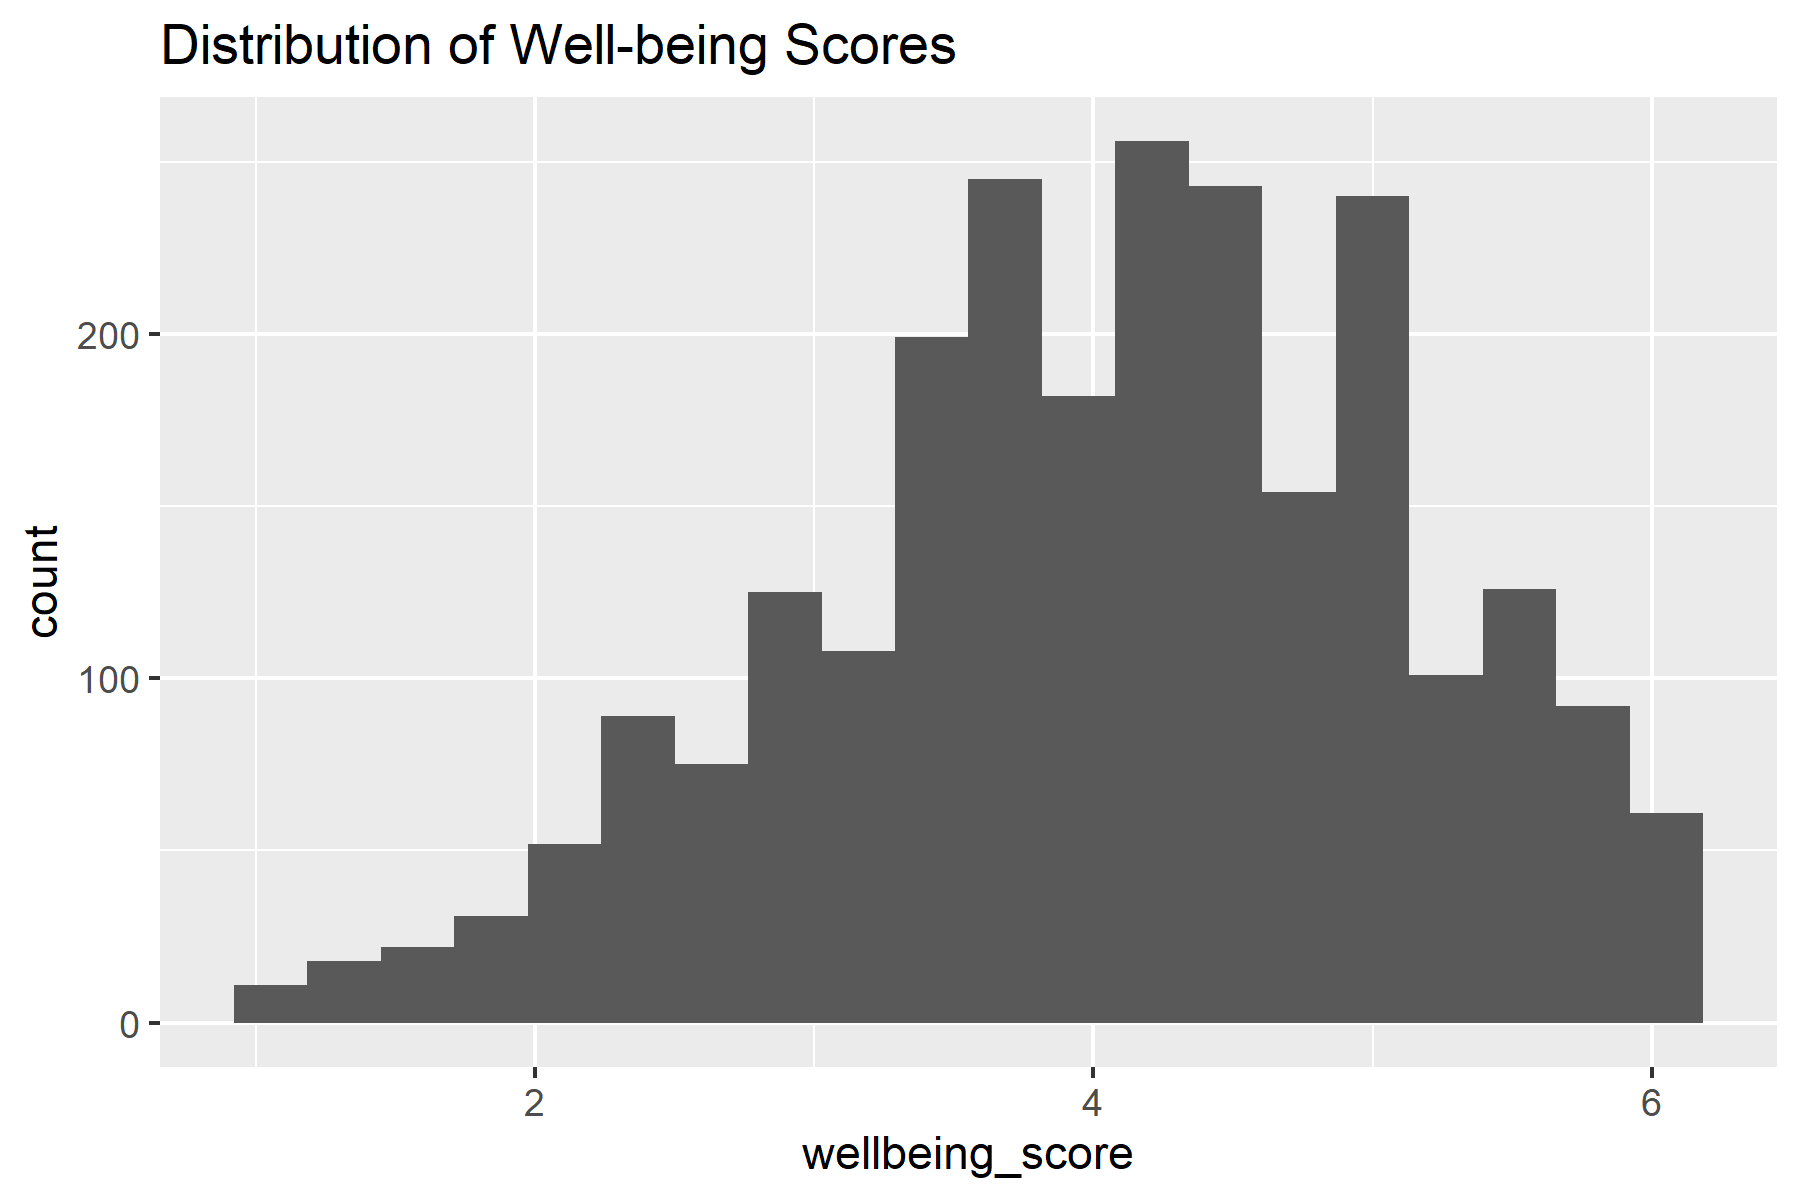
\includegraphics[width=\columnwidth]{wellbeing_distribution.png}
\captionof{figure}{Distribution of the ten-item well-being score.}
\label{fig:wbdist}
\end{center}

\subsection{Education measures}
Educational attainment is represented by nine variables: the respondent's highest education level, highest grade completed, whether they have attended college, whether they are currently in college, their educational aspirations, their educational expectations, hours spent in education, and the education levels of their mother and father. These span the respondent's own schooling, their forward-looking educational intentions, and parental (background) education.

\subsection{Missing data}
Listwise deletion is used throughout. The nine education variables are fully observed in the working sample, so the education models retain all 2{,}434 respondents. The well-being score has four missing values, and the ten individual well-being items together have additional missingness, leaving 2{,}396 complete cases for the item-level well-being models. The combined model, which uses the well-being score together with the education variables, retains 2{,}430 respondents. Because the samples differ slightly across specifications, the combined model is estimated on a single common sample to ensure that comparisons are not contaminated by changing composition.

\section{Empirical Strategy}
I evaluate the predictive content of the two domains using four methods, chosen so that their strengths and weaknesses are complementary. The outcome in every case is the binary employment indicator.

\subsection{Logistic regression}
The interpretable benchmark is a logistic regression,
\begin{equation}
\Pr(\text{employed}_i = 1 \mid X_i) = \Lambda\!\left(\beta_0 + X_i'\beta\right),
\end{equation}
where $\Lambda(\cdot)$ is the logistic CDF and $X_i$ is the vector of predictors from one domain. Coefficients are reported on the log-odds scale, and model fit is summarized by the Akaike Information Criterion (AIC), which penalizes added parameters and thus allows fit comparisons across domains with different numbers of predictors.

\subsection{Classification trees}
A classification tree (CART) recursively partitions respondents on the predictors to form homogeneous groups. Trees impose no linearity or additivity and are fully interpretable: the splits reveal which variables and thresholds separate the employed from the non-employed. A tree that produces no splits is itself informative---it indicates that no single predictor or interaction cleanly distinguishes the two groups.

\subsection{Random forests}
A random forest averages many trees grown on bootstrap samples with randomized splits. It captures nonlinearities and high-order interactions and yields two useful outputs: an out-of-bag (OOB) error estimate, which approximates out-of-sample accuracy, and variable-importance measures (mean decrease in accuracy and in Gini impurity) that rank predictors by their contribution. Each forest is grown with 500 trees.

\subsection{LASSO}
The LASSO estimates a penalized logistic regression,
\begin{equation}
\hat\beta = \arg\min_{\beta}\left\{-\ell(\beta) + \lambda \sum_{j} |\beta_j|\right\},
\end{equation}
where $\ell(\beta)$ is the log-likelihood and $\lambda$ governs the strength of the $\ell_1$ penalty, which shrinks coefficients toward zero and sets many exactly to zero. The penalty is chosen by cross-validation. I report two standard choices: $\lambda_{\min}$, which minimizes cross-validated deviance, and the more conservative $\lambda_{1se}$, the largest penalty within one standard error of the minimum. The number of variables surviving $\lambda_{1se}$ is a stringent measure of how much robust signal a domain contains.

\subsection{Does well-being add anything to education?}

The combined model refines the domain comparison by asking whether well-being contributes predictive information once education is held constant. In the combined logistic regression, the well-being coefficient increases from 0.049 in the bivariate model to 0.080 after controlling for education—a classic suppression pattern—but remains only marginally significant ($p = 0.053$). The AIC improves only slightly (3053.5 to 3051.7), and the likelihood-ratio test is borderline ($p = 0.052$).

Thus, while well-being shows a modest conditional association with employment once education is accounted for, the effect is small and statistically fragile. Education remains the dominant predictor, and well-being adds at most a weak secondary contribution.


\section{Results}

\subsection{Well-being predictors}

Well-being remains a weak predictor of employment under every method, even after correcting the tree procedure to evaluate performance on held-out data. In the logistic regression of employment on the well-being score alone, the coefficient is small and positive (0.049, standard error 0.039) and statistically insignificant ($p = 0.21$). The model's AIC of 3319.9 indicates poor fit relative to the education model.

Using a proper 70/30 train/test split, the well-being classification tree produces only a few shallow splits, and its predictive performance is weak: the test-set accuracy is just 55.1\%, barely above the naive baseline of always predicting the majority class (57\%). The splits that do appear—primarily on trusting relationships, managing responsibilities, and perceptions of whether people are good—do not form a stable or interpretable structure, and the terminal nodes differ only modestly in employment rates.

The random forest confirms this lack of signal. Its out-of-bag error rate is 48.2\%, essentially equivalent to guessing. Although a few items (satisfaction, managing responsibilities, trusting relationships) appear slightly more important than others, the absolute magnitudes of the importance measures are small, and the forest does not extract meaningful predictive structure.

The LASSO reinforces this conclusion. At $\lambda_{\min}$ a handful of items enter with small coefficients, but under the conservative $\lambda_{1se}$ rule every well-being variable is shrunk to zero. In short, even with corrected out-of-sample evaluation, the ten well-being indicators contain essentially no predictive information about young-adult employment.


The classification tree is even more emphatic: it produces \emph{no splits at all}, collapsing to the root node. No well-being item, alone or in combination, separates the employed from the non-employed cleanly enough to warrant a partition. The random forest tells the same story. Its out-of-bag error rate is 48.2\%, which is actually \emph{worse} than the roughly 43\% error obtained by naively predicting ``employed'' for every respondent. In other words, the ten well-being items contain no usable predictive signal for employment. The variable-importance plot does rank some items above others---satisfaction, managing responsibilities, and trusting relationships appear modestly more important---but in absolute terms the predictive contribution is negligible.

The LASSO confirms this pattern. At $\lambda_{\min}$ a handful of items survive with small coefficients (satisfaction, interest in life, happiness, and managing responsibilities entering positively; community and ``society is getting better'' entering negatively), but at the conservative $\lambda_{1se}$ \emph{every} well-being variable is shrunk to zero. The model that minimizes cross-validated error is barely distinguishable from one with no predictors. Taken together, the four methods agree that well-being, measured this way, does not predict young-adult employment.

\subsection{Education predictors}

Education continues to show strong and stable predictive power across all methods. In the education-only logistic regression, several variables are highly significant. Prior college attendance (coefficient 0.356) and current college enrollment (0.482) are both strongly positive and highly significant ($p < 0.001$). Educational expectations ($-0.073$), hours in education ($-0.0007$), and father's education ($-0.0035$) are also significant, as are highest education level and educational aspirations at conventional levels. The model's AIC of 3066.3 is far lower than the well-being model's 3319.9, indicating substantially better fit.

The corrected classification tree, now evaluated using a 70/30 train/test split, again reveals meaningful structure. The tree splits repeatedly on education hours, educational expectations, current college enrollment, highest education, and parental education. The resulting terminal nodes vary widely in employment rates, and the model achieves a test-set accuracy of 69.2\%, a substantial improvement over the well-being tree and well above the naive baseline.

The random forest corroborates these findings. Its most important predictors—current college enrollment, highest education, and hours in education—align with human-capital theory, and the forest extracts clear nonlinear structure from the education block.

The LASSO also retains a robust set of predictors. At $\lambda_{\min}$ all nine education variables survive, and even under the conservative $\lambda_{1se}$ penalty, seven variables remain active. This stands in sharp contrast to the well-being LASSO, which retains none. Across all methods, education consistently demonstrates strong predictive content.


\begin{center}
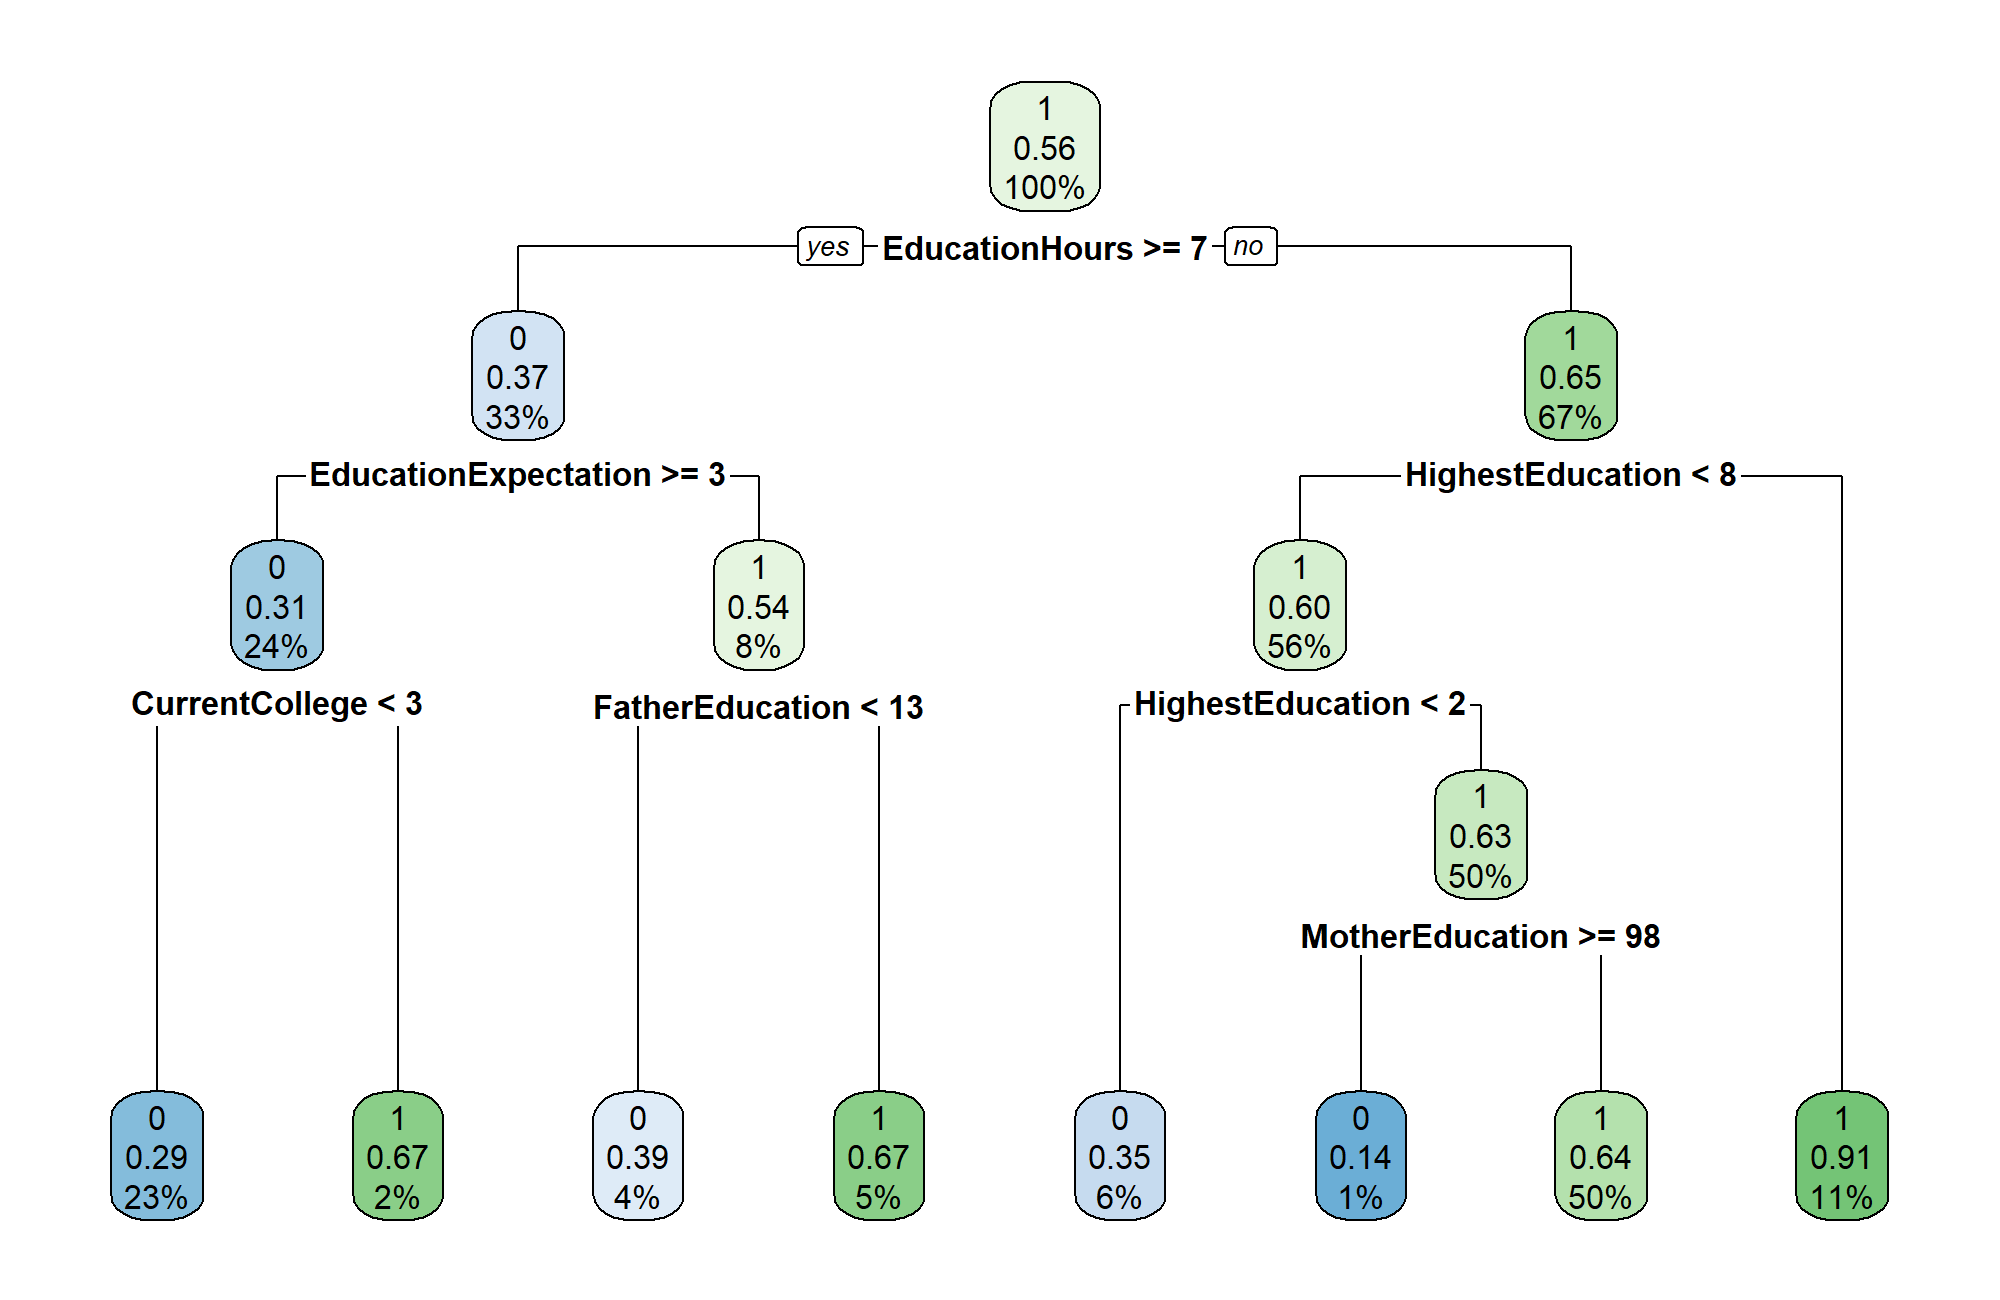
\includegraphics[width=\columnwidth]{education_tree.png}
\captionof{figure}{Classification tree for the education predictors. Each node reports the predicted class, the employment rate, and the share of the sample.}
\label{fig:edtree}
\end{center}

\subsection{Domain comparison}
\subsection{Domain comparison}

Table~\ref{tab:compare} summarizes the head-to-head comparison across methods. Education outperforms well-being on every meaningful criterion: a much lower logistic AIC, a tree that produces multiple stable splits and achieves substantially higher test-set accuracy, and a LASSO that retains a large subset of predictors even under strong regularization. The well-being domain, by contrast, yields an insignificant logistic coefficient, a weak and shallow tree with poor test-set accuracy, a random forest no better than guessing, and a LASSO that discards all variables at $\lambda_{1se}$.

The one metric on which well-being superficially appears competitive—random-forest training accuracy—is misleading, as random forests overfit the training data. The out-of-bag error rate (48\%) is the correct measure and shows no predictive value. Once proper out-of-sample evaluation is used, the superiority of the education domain is unambiguous.


\begin{center}
\captionof{table}{Model comparison: well-being vs.\ education predictors.}
\label{tab:compare}
\footnotesize
\begin{tabular}{lcc}
\toprule
Criterion & Well-being & Education \\
\midrule
Logistic regression AIC      & 3319.9 & 3066.3 \\
CART splits                  & 0      & 7      \\
LASSO variables ($\lambda_{1se}$) & 0 & 7      \\
RF training accuracy         & 0.955  & 0.918  \\
\bottomrule
\end{tabular}
\end{center}

The one criterion on which the two domains look similar, and on which well-being even appears slightly ahead, is random-forest accuracy (0.955 vs.\ 0.918). This comparison is misleading and should be discounted. These are \emph{training} accuracies computed by predicting the same data the forest was grown on, which random forests memorize; they do not reflect out-of-sample performance. The honest measure of the well-being forest's performance is its out-of-bag error of 48\%, which, as noted, is no better than guessing. The inflated training accuracy is an artifact, not evidence that well-being predicts employment. The AIC, tree, and LASSO comparisons uniformly favor education.

\begin{center}
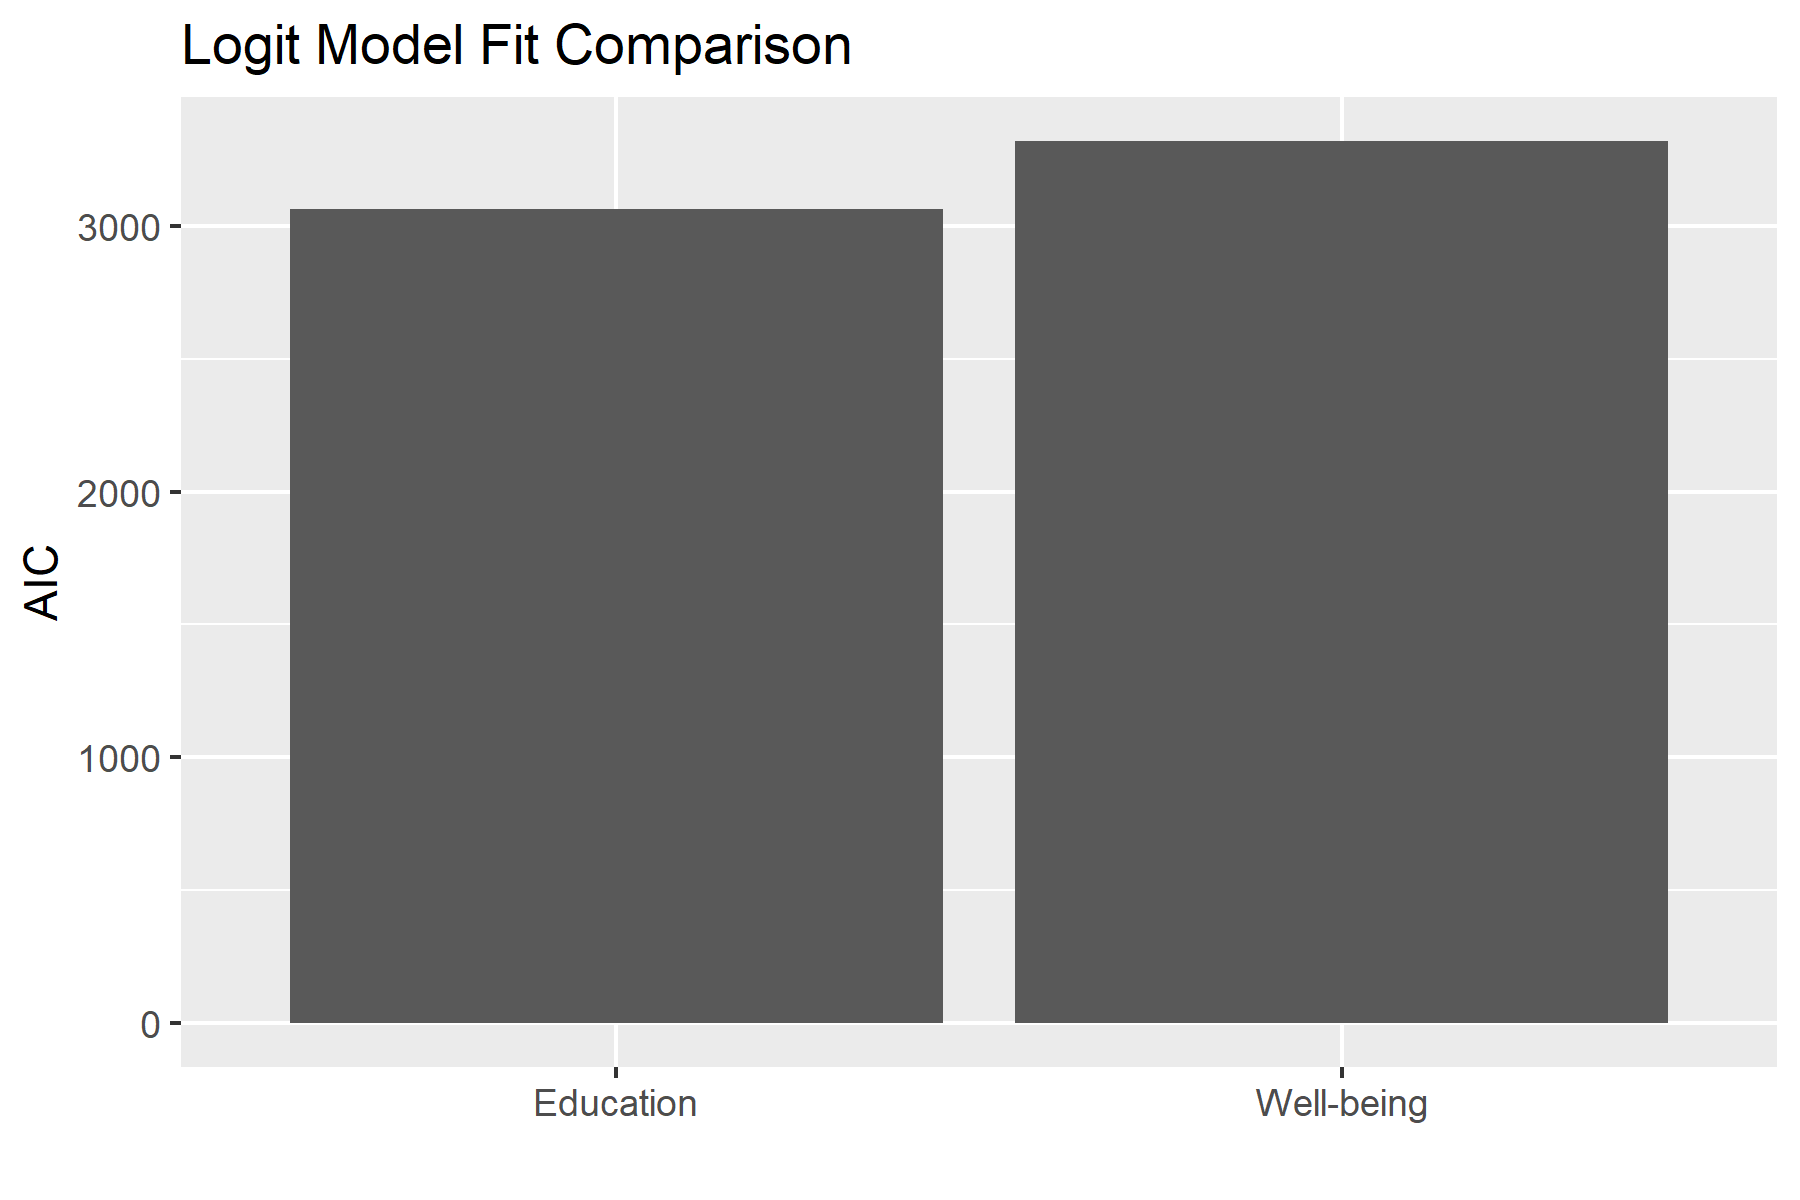
\includegraphics[width=\columnwidth]{logit_aic_comparison.png}
\captionof{figure}{Logistic-regression fit (AIC; lower is better) for the well-being and education models.}
\label{fig:aic}
\end{center}

\subsection{Does well-being add anything to education?}
The domain comparison establishes that well-being is weak on its own. The combined model asks the sharper question: does well-being contribute once education is controlled? In the combined model, the well-being coefficient is 0.080 with a $p$-value of 0.053, while the education variables retain essentially the same magnitudes and significance as in the education-only model. Adding well-being lowers the AIC only slightly, from 3053.5 to 3051.7, and the likelihood-ratio test against the education-only model yields $p = 0.052$. All three diagnostics place well-being right at the conventional significance threshold.

The most striking feature is that the well-being coefficient \emph{grew} after controlling for education, rising from 0.049 in the bivariate model to 0.080 in the combined model (Figure~\ref{fig:wbcoef}). This is a classic suppression pattern: education was masking the well-being--employment relationship, and holding it constant uncovers a somewhat larger positive association. The direction is therefore opposite to the usual case in which a weak predictor is rendered insignificant by adding controls. Substantively, the coefficient of 0.080 implies that a one-point increase in the well-being score (on its 1--6 scale) is associated with about an 8\% increase in the odds of employment-a modest effect that is statistically borderline rather than clearly significant.

\begin{center}
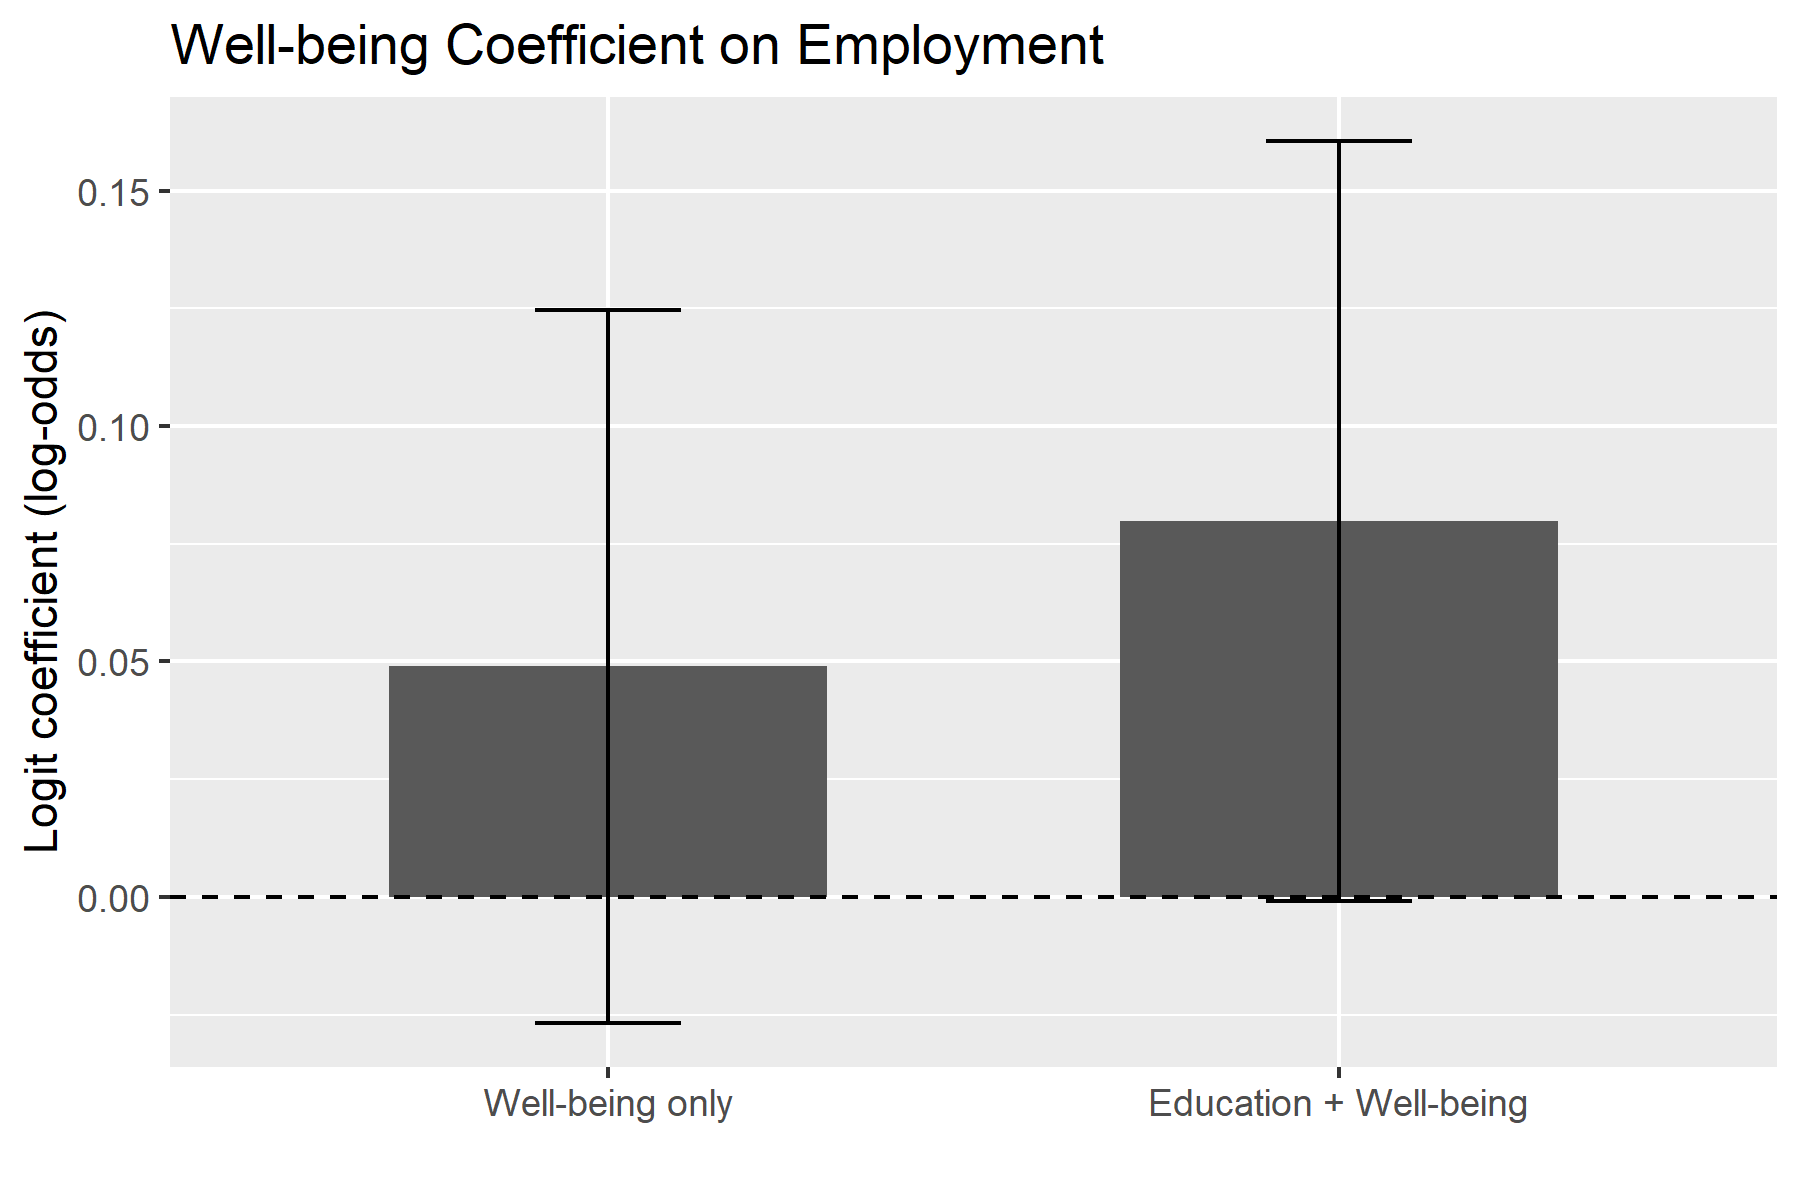
\includegraphics[width=\columnwidth]{wellbeing_coef_comparison.png}
\captionof{figure}{Well-being coefficient before and after controlling for education, with 95\% confidence intervals. The effect strengthens but its interval still reaches zero.}
\label{fig:wbcoef}
\end{center}

\section{Discussion and Conclusion}
Across logistic regression, classification trees, random forests, and the LASSO, the evidence points consistently in one direction: among young adults in PSID-TAS 2023, educational characteristics are strong and stable predictors of current employment, while subjective well-being is not. Education produces a well-fitting logistic model, a richly branching tree, an important set of random-forest predictors, and a robust set of LASSO-selected variables. Well-being produces an insignificant logistic coefficient, a tree with no splits, a forest no better than guessing, and a LASSO that discards every indicator. The contrast is hard to miss.

The combined model refines rather than overturns this conclusion. Well-being does carry a small positive association with employment that becomes visible only after education is held constant---the suppression pattern in Figure~\ref{fig:wbcoef}. One interpretation is that education is correlated with both well-being and employment in offsetting ways, so that the raw well-being--employment relationship understates the conditional one. Even so, the conditional effect is small and lands just short of conventional significance, so the appropriate summary is that well-being is, at most, a weak and secondary predictor once education is taken into account. The headline result (education dominates) is unchanged.

Several limitations qualify these findings. First, the analysis is a single cross-section, so it describes predictive associations, not causal effects; in particular, employment and well-being may influence one another, and the direction cannot be resolved here. Second, the outcome and predictors are self-reported survey measures subject to reporting error. Third, listwise deletion discards incomplete cases, and items with more missingness contribute less. Fourth, the random-forest accuracies in the comparison table are in-sample and overstate true performance, especially for well-being---the out-of-bag error is the more honest figure and would be the natural target for future out-of-sample validation. Fifth, the education variables are treated as continuous even though several are ordinal or categorical, and the well-being index averages ten items that tap distinct hedonic and eudaimonic dimensions; disaggregating those dimensions, or modeling the categorical education measures with appropriate indicators, could sharpen the analysis. Finally, the models omit demographic controls such as age, sex, and income; including them would clarify whether the education and well-being associations are partly compositional.

Despite these caveats, the practical message is clear and robust to the modeling choice. For predicting which young adults are employed, what they are doing educationally (i,e. whether they have attended or are enrolled in college, and how their schooling is structured) matters far more than how they feel about their lives. Well-being may still be valuable for other outcomes and over longer horizons, but as a short-run predictor of employment among young adults it adds little beyond the human-capital measures that have long anchored labor-economic models.

\end{multicols}

\end{document}
